\documentclass[]{article}
\newcommand{\FileDepth}{../../..}
\usepackage[letterpaper, landscape, margin=0.5cm]{geometry}
\usepackage[T1]{fontenc}
\usepackage{textcomp}%Not strictly necessary, but gives \textmu command for "micro."
\usepackage{fancyhdr}
\usepackage{amsmath}
\usepackage{amssymb}
\usepackage{graphicx}
\usepackage{xcolor}
\usepackage{tikz}
\usetikzlibrary{calc}
\usepackage[shortlabels]{enumitem}
\usepackage{multicol}
\usepackage{vwcol}
\usepackage{hyperref}
\usepackage{wrapfig}
%opening
\newcommand{\SecType}{L}
\newcommand{\Week}{12}
\title{PH 211 Lecture \Week}
\author{Benjamin Bauml}
\date{Summer 2024}

\newcommand{\Purpose}{4}
\newcommand{\DefOnly}{0}

% Version 2024-06-14
% Changes
% 2024-02-21 Added xstring package to enable smooth implementation of new \ModePage command.
% 2024-04-27 Set up to split activities and formatting aspects into separate files. Removed dependence on xcomment. Added an automatic counter to number the activities in a problem set.
% 2024-05-19 Revised old format for \TeachingTips command, which did not support \DefOnly.
% 2024-06-14 Added Repurpose environment to allow mixing of different purpose levels in the same document.
\usepackage{tcolorbox}
\usepackage{xstring}
% You will want the following four lines in your document (the last two uncommented):
% For Assignment, leave Purpose as 1. For Worksheet, set to 2. For Student Solution, set to 3. For Teacher Solution, set to 4.
% If you want keep the pieces from being called manually, set DefOnly to 0.
%\newcommand{\Purpose}{4}
%\newcommand{\DefOnly}{1}
\newcommand{\Exclusion}{0}
\newcommand{\PageTurn}{0}
\newcommand{\GrayProb}{0}
\newcommand{\Tipsy}{0}

% Assignment
\if\Purpose1
\renewcommand{\Exclusion}{1}
\fi
% Worksheet
\if\Purpose2
\renewcommand{\Exclusion}{1}
\renewcommand{\PageTurn}{1}
\fi
% Student Solution
\if\Purpose3
\renewcommand{\PageTurn}{1}
\renewcommand{\GrayProb}{1}
\fi
% Teaching Copy
\if\Purpose4
\renewcommand{\PageTurn}{1}
\renewcommand{\GrayProb}{1}
\renewcommand{\Tipsy}{1}
\fi

\newenvironment{Repurpose}[1]{
\renewcommand{\Purpose}{#1}
\renewcommand{\Exclusion}{0}
\renewcommand{\PageTurn}{0}
\renewcommand{\GrayProb}{0}
\renewcommand{\Tipsy}{0}
% Assignment
\if\Purpose1
\renewcommand{\Exclusion}{1}
\fi
% Worksheet
\if\Purpose2
\renewcommand{\Exclusion}{1}
\renewcommand{\PageTurn}{1}
\fi
% Student Solution
\if\Purpose3
\renewcommand{\PageTurn}{1}
\renewcommand{\GrayProb}{1}
\fi
% Teaching Copy
\if\Purpose4
\renewcommand{\PageTurn}{1}
\renewcommand{\GrayProb}{1}
\renewcommand{\Tipsy}{1}
\fi
}{}

\def \NewQ {0}
\def \PForce {0}
\newcommand{\MaybePage}[1]{
	\def \PForce {#1}
	\if\PForce1
	\newpage
	\else
	\if\NewQ0
	\gdef \NewQ {\PageTurn}
	\else
	\newpage
	\fi
	\fi
}

\newcommand{\ModePage}[1]{
	\IfSubStr{#1}{\Purpose}{\newpage}{}
}

\newcounter{ActNumber}
\setcounter{ActNumber}{0}

\newcommand{\Problem}[4][0]{%The first argument is optional, and if it is set to 1, the \newpage will be forced. The second argument is the name of the activity, the third is the command the activity is stored as, and the fourth is the actual problem statement.
\newcommand{#3}{
\MaybePage{#1}
\addtocounter{ActNumber}{1}
\section*{\SecType\Week-\theActNumber: #2}
\if\GrayProb1
\begin{tcolorbox}[colback=lightgray,colframe=lightgray,sharp corners,boxsep=1pt,left=0pt,right=0pt,top=0pt,bottom=0pt,after skip=2pt]
\else
\begin{tcolorbox}[colback=white,colframe=white,sharp corners,boxsep=1pt,left=0pt,right=0pt,top=0pt,bottom=0pt,after skip=2pt]
\fi
#4
\end{tcolorbox}\noindent
}
\if\DefOnly0
\else
#3
\fi
}
	
\newcommand{\ProblemSub}[3][0]{%The first argument is optional, and if a string of numbers is entered into it, it will force a \newpage in any \Purpose that shows up in the string. For example, "13" would lead to the newpage being forced in modes 1 and 3. The second is the command the activity is stored as, and the third is the actual problem statement.
\newcommand{#2}{
\ModePage{#1}
\if\GrayProb1
\begin{tcolorbox}[colback=lightgray,colframe=lightgray,sharp corners,boxsep=1pt,left=0pt,right=0pt,top=0pt,bottom=0pt,after skip=2pt]
\else
\begin{tcolorbox}[colback=white,colframe=white,sharp corners,boxsep=1pt,left=0pt,right=0pt,top=0pt,bottom=0pt,after skip=2pt]
\fi
#3
\end{tcolorbox}\noindent
}
\if\DefOnly0
\else
#2
\fi
}
		
\newcommand{\Solution}[2]{%The first argument is the command the solution is stored as, and the second is the actual solution.
\newcommand{#1}{
\if\Exclusion0
#2
\fi
}
\if\DefOnly0
\else
#1
\fi
}
		
\newcommand{\ProblemFig}[2]{%The first argument is the command the figure is stored as, and the second is the actual figure.
\newcommand{#1}{
\begin{figure}[h]
#2
\end{figure}
}
\if\DefOnly0
\else
#1
\fi
}

\newcommand{\TeachingTips}[2]{%The first argument is the command the tip is stored as, and the second is the actual tip.
\newcommand{#1}{
\if\Tipsy1
\begin{tcolorbox}[colback=lightgray,colframe=black]
#2
\end{tcolorbox}
\fi
}
\if\DefOnly0
\else
#1
\fi
}
\usepackage[absolute]{textpos}
% This package relies on Assignment Format 2024-06-14 or later to work. It is recommended that the Purpose and DefOnly commands be given as such:
%\newcommand{\Purpose}{4}
%\newcommand{\DefOnly}{0}
% Activities need to be entered outside of the TeacherMargin and PresentSpace environments, otherwise they will be defined only locally. They can even go in the preamble.
\newenvironment{TeacherMargin}{\begin{textblock*}{10.8cm}(0.5cm,0.5cm)
\small}{\end{textblock*}
\hspace{0.1cm}}
\newenvironment{PresentSpace}{\begin{textblock*}{0.3cm}(26.85cm,9.35cm)
--
\end{textblock*}
\begin{textblock*}{0.3cm}(26.85cm,18.7cm)
--
\end{textblock*}
\begin{textblock*}{0.3cm}(26.85cm,12.24cm)
	--
\end{textblock*}
\begin{textblock*}{15.6cm}(11.8cm,0.5cm)
\begin{Repurpose}{1}
\Large}{\end{Repurpose}
\end{textblock*}
\hspace{0.1cm}}

\newcommand{\FBDaxes}[3]{
	\begin{scope}[shift={(#1)},rotate=#2]
		% x-axis
		\draw[thick,->] (-2,0) -- (2,0);
		\node[anchor=west] at (2,0) {$x$};
		% y-axis
		\draw[thick,->] (0,-2) -- (0,2);
		\node[anchor=west] at (0,2) {$y$};
		\coordinate (#3) at (0,0);
	\end{scope}
}
\newcommand{\FBDvectorMA}[4]{
	\begin{scope}[shift={(#1)}]
		\coordinate (#4tip) at ({#2*cos(#3)},{#2*sin(#3)});
		\draw[ultra thick,blue,->] (#1) -- (#4tip);
	\end{scope}
}
\newcommand{\FBDvectorXY}[3]{
	\begin{scope}[shift={(#1)}]
		\coordinate (#3tip) at (#2);
		\draw[ultra thick,blue,->] (0,0) -- (#3tip);
	\end{scope}
}
\newcommand{\FBDdot}[1]{
	\filldraw[black] (#1) circle (3pt);
}
%\newcommand{\MVec}[3][0]{%Creates a momentum vector of length #3 centered at #2 and rotated #1 degrees counterclockwise.
	\begin{scope}[rotate=#1,shift={(#2)}]
		\draw[->,thick] ({-#3/2},0) -- ({#3/2},0);
	\end{scope}
}
\newcommand{\MDot}[1]{%Creates a dot at #1 to represent a zero vector.
	\filldraw (#1) circle (1pt);
}
\newcommand{\MVDRows}[2][4.5]{%Creates the rows (initial, delta, final) of a momentum vector diagram. The optional argument determines the width of the table, and defaults to a good length for three columns (two objects and the total system). The non-optional argument gives a coordinate name (not displayed) to the diagram.
	\begin{scope}
		%\draw[thick] (0,5.5) -- (0,0);
		\draw[thick] (-1,4.5) -- (#1,4.5);
		\node at (-0.5,3.75) {$\vec{p}_{i}$};
		\draw[thick] (-1,3) -- (#1,3);
		\node at (-0.5,2.25) {$\Delta\vec{p}$};
		\draw[thick] (-1,1.5) -- (#1,1.5);
		\node at (-0.5,0.75) {$\vec{p}_{f}$};
		\coordinate (#2) at (0,5);
	\end{scope}
}
\newcommand{\MVDCol}[4][0.75]{%Creates a column for an object in a momentum vector diagram. The first (non-optional) argument is the coordinate name (not displayed) of the column, while the second is the displayed column header. The first argument also names the three entries down the column. The third argument anchors the column, so it should either be the coordinate name of the MVD (for the first column) or the coordinate name of the previous column. The optional argument indicates how far the center of the column should be from the previous column's edge, and defaults to 0.75
	\begin{scope}[shift={(#4)}]
		\node at (#1,0) {#3};
		%\draw[thick] ({#1*2},0.5) -- ({#1*2},-5);
		\draw[thick] (0,0.5) -- (0,-5);
		\coordinate (#2init) at (#1,-1.25);
		\coordinate (#2delt) at (#1,-2.75);
		\coordinate (#2fin) at (#1,-4.25);
		\coordinate (#2) at ({#1*2},0);
	\end{scope}
}

%\input{\FileDepth/Activities/Activity_One/Activity_One.tex}
%\input{\FileDepth/Activities/Activity_Two/Activity_Two.tex}

\begin{document}
\begin{TeacherMargin}
\noindent\textbf{Ungrading Prompts}
\begin{enumerate}[(1)]
	\item Assemble all of your work for the term (Get-Ready assignments, weekly homeworks, lab reports, project submissions).
	\item Read through everything (your work, your reflections, the feedback you received).
	\item Answer the following questions based on your review of your work:
	\begin{enumerate}[(a)]
		\item What portions of your work are you most proud of, and why?
		\item Through your work, what did you learn the most about during the term?
		\item What areas of your work would benefit the most from further development?
	\end{enumerate}
	\item How many class sessions were you able to attend?
	\begin{enumerate}[(a)]
		\item If you missed any class sessions, were you able to complete the work for class at a distance?
		\begin{enumerate}[(i)]
			\item If you could not complete all classwork at a distance, please explain why this was the case.
		\end{enumerate}
	\end{enumerate}
	\item Describe your level of engagement during class.
	\item Roughly how much of the readings for class did you complete as assigned?
	\item Were you able to turn in all of your assignments on time?
	\begin{enumerate}[(a)]
		\item If not, please explain why you were not able to do so.
	\end{enumerate}
	\item Reflect on your experience with ungrading; what was your experience with this process at the beginning, middle, and end of the class?
	\item Please suggest a grade for yourself and provide a brief rationale for your suggestion.
\end{enumerate}
\end{TeacherMargin}
\begin{PresentSpace}
\begin{center}
	\huge Lecture \Week: Force Analysis and Special Cases
\end{center}
\vspace{0.5cm}
\underline{Announcements}
%\begin{multicols}{2}
\begin{itemize}
	\item Mid-Term Ungrading due Saturday at 11:59 p.m.
	\begin{itemize}
		\item Prompts for Ungrading are in the Syllabus, the Mid-Term Ungrading assignment, and in these lecture notes.
		\item Review all of your work and feedback so far, discuss your work, your attendance, and your engagement, then propose a grade for yourself.
		\item Citing and quoting your work and feedback as evidence is good.
		\item Suggested minimum length of 2 pages.
	\end{itemize}
	\item Homework 4 assessment completed
	\begin{itemize}
		\item The Angled Block and the Calculate part of The Penny in the Elevator were not evaluated.
		\item Compare your work against the solution. If you have questions or want more feedback, take your work into the Wormhole or office hours.
	\end{itemize}
\end{itemize}
%\end{multicols}
\end{PresentSpace}
\newpage
\begin{TeacherMargin}

\end{TeacherMargin}
\begin{PresentSpace}
\vspace{-10pt}
\section*{A Model for Interactions}
\vspace{-10pt}
\begin{itemize}
	\item Quantities
	\begin{itemize}
		\item Mass \quad $m$ \qquad \textbf{--} Force \quad $\vec{F}$
		%\item Force \quad $\vec{F}$
	\end{itemize}
	\item Laws
	\begin{itemize}
		\item Net force is proportional to acceleration: \\
		$\vec{F}^{net}=m\vec{a}$
		\item Forces come in pairs: $\vec{F}_{AB} = -\vec{F}_{BA}$
	\end{itemize}
	\item Asssumptions
	\begin{itemize}
		\item We can treat multiple objects as a system.
		\item All forces act as if on the center of the system.
	\end{itemize}
\end{itemize}
\end{PresentSpace}
\begin{textblock*}{5cm}(22cm,1.34cm)
\Large
\begin{itemize}
	\item Diagram
\end{itemize}
\centering
\begin{tikzpicture}
	\FBDbox{0,0}{0}{box}{}
	\FBDvectorXY{boxtrq}{0,1.2}{FM}
	\node[anchor=west] at (FMtip) {$\vec{F}^{M}_{BI}$};
	\FBDvectorXY{boxtlq}{0,1.7}{FN}
	\node[anchor=east] at (FNtip) {$\vec{F}^{N}_{BG}$};
	\FBDvectorXY{boxrcent}{1.75,0}{FKF}
	\node[anchor=south] at (FKFtip) {$\vec{F}^{kf}_{BG}$};
	\FBDvectorXY{boxbcent}{0,-2.9}{FG}
	\node[anchor=west] at (FGtip) {$\vec{F}^{g}_{BE}$};
\end{tikzpicture}
\end{textblock*}
\newpage
\begin{TeacherMargin}

\end{TeacherMargin}
\begin{PresentSpace}
\vspace{-10pt}
\section*{Solving Problems Using Forces}
\vspace{-10pt}
\begin{itemize}
	\item Identify a system.
	\item Identify the (external) forces acting on the system.
	\begin{itemize}
		\item Draw a free-body diagram.
	\end{itemize}
	\item Identify the acceleration (\textbf{not a force}).
	\begin{itemize}
		\item Static/dynamic equilibrium (acceleration = 0)
		\item Dynamics (acceleration not 0)
	\end{itemize}
	\item Use the laws of motion.
	\item Reflect on your answer (check units and evaluate special cases).
\end{itemize}
\end{PresentSpace}
\newpage
\begin{TeacherMargin}

\end{TeacherMargin}
\begin{PresentSpace}
\vspace{-10pt}
\section*{Special-Case Analysis}
\vspace{-10pt}
After you solve for a quantity:
\begin{itemize}
	\item Choose a case that is \textbf{special}, not arbitrary.
	\item Figure out what your quantity \textbf{should} be in the case you chose.
	\item Identify the value of one or more other quantities that corresponds to your \textbf{case}.
	\item Evaluate your answer in the special case.
	\item Check whether or not your symbolic answer for the case matches what you expected the answer should be.
\end{itemize}
\end{PresentSpace}
\newpage
\begin{TeacherMargin}
\noindent Let's call the rope on the left rope 1, and the rope on the right rope 2.
\begin{center}
	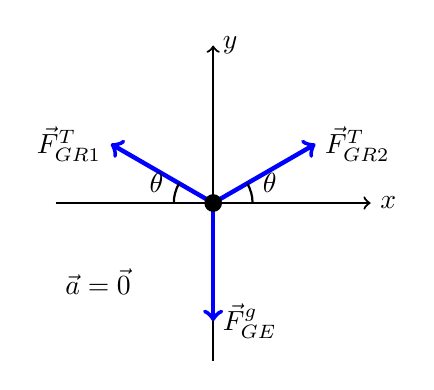
\begin{tikzpicture}
		\FBDaxes{0,0}{0}{axes}
		\FBDvectorMA{axes}{1.5}{30}{FTR}
		\node[anchor=west] at (FTRtip) {$\vec{F}^{T}_{GR2}$};
		\draw[thick] (0.5,0) node[anchor=south west] {$\theta$} arc (0:30:0.5);
		\FBDvectorMA{axes}{1.5}{150}{FTL}
		\node[anchor=east] at (FTLtip) {$\vec{F}^{T}_{GR1}$};
		\draw[thick] (-0.5,0) node[anchor=south east] {$\theta$} arc (180:150:0.5);
		\FBDvectorXY{axes}{0,{-3*sin(30)}}{FG}
		\node[anchor=west] at (FGtip) {$\vec{F}^{g}_{GE}$};
		\node[anchor=west] at (-2,-1) {$\vec{a}=\vec{0}$};
		\FBDdot{axes}
	\end{tikzpicture}
\end{center}
\[
\vec{F}^{net} = m\vec{a} = \vec{0}
\]
From the $x$-component of the net force, we find that the balance of forces and the equal angles require the tensions to be the same. This then can be used to simplify the $y$-component of the net force and solve for this one tension.
\begin{align*}
	0 & = F^{net}_{x} & 0 & = F^{net}_{y} \\
	& = -F^{T}_{GR1}\cos\theta & 0 & = F^{T}_{GR1}\sin\theta + F^{T}_{GR2}\sin\theta - F^{g} \\
	& \quad + F^{T}_{GR2}\cos\theta & 0 & = 2F^{T}\sin\theta - F^{g} \\
	F^{T}_{GR1}\cos\theta & =  F^{T}_{GR2}\cos\theta & 2F^{T}\sin\theta & = F^{g} = mg \\
	F^{T}_{GR1} & =  F^{T}_{GR2} = F^{T} & F^{T} & = \frac{mg}{2\sin\theta} \\
\end{align*}
\textbf{Special Cases}
\begin{center}
	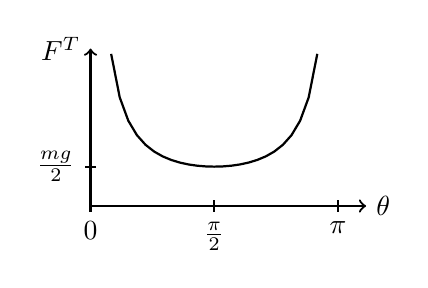
\begin{tikzpicture}
		\draw[thick,<->] (0,2) node[anchor=east] {$F^{T}$} -- (0,0) -- (3.5,0) node[anchor=west] {$\theta$};
		\draw[thick] (0,2pt) -- (0,-2pt) node[anchor=north] {0};
		\draw[thick] ({pi/2},2pt) -- ({pi/2},-2pt) node[anchor=north] {$\frac{\pi}{2}$};
		\draw[thick] ({pi},2pt) -- ({pi},-2pt) node[anchor=north] {$\pi$};
		\draw[thick,domain=15:165,variable=\th] plot ({pi*\th/180},{1/(2*sin(\th))});
		\draw[thick] (2pt,0.5) -- (-2pt,0.5) node[anchor=east] {$\frac{mg}{2}$};
	\end{tikzpicture}
\end{center}
\begin{itemize}
	\item If the ropes are vertical ($\theta=\pi/2$), then they both hang straight down, and they should each support half of the gymnast's weight (they don't need anything extra to pull in the $x$-direction).
	\begin{itemize}
		\item $F^{T} = \frac{mg}{2\sin(\pi/2)} = \frac{mg}{2}$
	\end{itemize}
	\item If the ropes are horizontal with no $y$-component, then they need to be extremely taut. In fact, it is impossible for a rope with weight in the middle not to sag a bit (because the ropes need to be tilted to exert an upward force on the suspended mass), so it should require an unrealistic amount of force to make the ropes completely flat.
	\begin{itemize}
		\item $F^{T} = \frac{mg}{2\sin(0)} = \frac{mg}{0} = \infty$
	\end{itemize}
	\item If the gymnast has no mass, then the ropes don't need to exert any force. $F^{T} = \frac{(0\text{ kg})g}{2\sin\theta} = 0$
\end{itemize}
\end{TeacherMargin}
\begin{PresentSpace}
\vspace{-10pt}
\section*{L\Week-1: The Gymnast}
\vspace{-10pt}
A gymnast of mass $m$ is training using two \\
ropes attached to the ceiling, as shown in \\
the figure. The gymnast is suspended at rest.
\begin{itemize}
	\item Identify and determine the magnitude of all \\
	forces acting on the gymnast.
	\item What special case(s) do you want to choose for \\
	this problem? Why?
	\item Try out at least one special case. (Make sure you \\
	know what the answer \textit{should} be in your case!)
\end{itemize}
\end{PresentSpace}
\begin{textblock*}{5cm}(20cm,0cm)
\centering

\includegraphics[scale=2]{Gymnast_Suspended_with_Equal_Angles}
\end{textblock*}
\newpage
\begin{TeacherMargin}
\begin{center}
	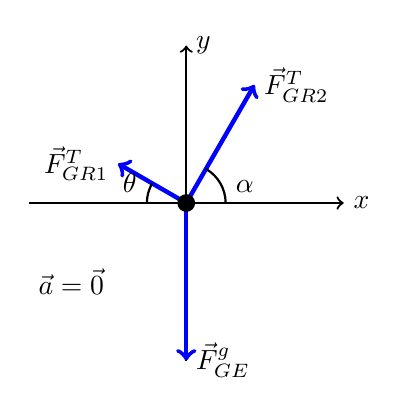
\begin{tikzpicture}
		\FBDaxes{0,0}{0}{axes}
		\FBDvectorMA{axes}{2*cos(30)}{60}{FTR}
		\node[anchor=west] at (FTRtip) {$\vec{F}^{T}_{GR2}$};
		\draw[thick] (0.5,0) node[anchor=south west] {$\alpha$} arc (0:60:0.5);
		\FBDvectorMA{axes}{1}{150}{FTL}
		\node[anchor=east] at (FTLtip) {$\vec{F}^{T}_{GR1}$};
		\draw[thick] (-0.5,0) node[anchor=south east] {$\theta$} arc (180:150:0.5);
		\FBDvectorXY{axes}{0,{-sin(30)-2*cos(30)*sin(60)}}{FG}
		\node[anchor=west] at (FGtip) {$\vec{F}^{g}_{GE}$};
		\node[anchor=west] at (-2,-1) {$\vec{a}=\vec{0}$};
		\FBDdot{axes}
	\end{tikzpicture}
\end{center}
\textbf{Left vs. Right} \\
Both tensions must have equal $x$-components, as the forces balance in the $x$-direction. We can relate the magnitudes of the $y$-components to the magnitudes of the $x$-components by
\begin{align*}
	|F^{T}_{GR1,y}| & = |F^{T}_{GR1,x}|\tan\theta, & |F^{T}_{GR2,y}| & = |F^{T}_{GR2,x}|\tan\alpha,
\end{align*}
and since the $x$-components are equal, this becomes
\[
\frac{|F^{T}_{GR1,y}|}{|F^{T}_{GR2,y}|} = \frac{\tan\theta}{\tan\alpha}.
\]
Since $\alpha>\theta$, we know that $\tan\alpha>\tan\theta$, and therefore $|F^{T}_{GR2,y}| > |F^{T}_{GR1,y}|$. This tells us that $F^{T}_{GR2} > F^{T}_{GR1}$. The left tension is less than the right tension.

\noindent\textbf{Special Case} \\
If you set $\theta=\alpha$, your equations for both tensions should simplify to what we found before: $F^{T} = \frac{mg}{2\sin\theta}$.
\end{TeacherMargin}
\begin{PresentSpace}
\vspace{-10pt}
\section*{L\Week-2: The Gymnast \textit{Reloaded}}
\vspace{-10pt}
What if the ropes were different angles?
\begin{itemize}
	\item Don't solve the problem yet!
	\item You have a problem like this on your \\
	homework.
	\item Do you expect the left tension to be \textit{greater than}, \\
	\textit{less than}, or \textit{equal to} the right tension?
	\item What special case could you evaluate after you \\
	solve this problem to check if your answer is right?
\end{itemize}
\end{PresentSpace}
\begin{textblock*}{5cm}(20cm,0cm)
\centering

\includegraphics[scale=2]{Gymnast_Suspended_with_Unequal_Angles}
\end{textblock*}
\newpage
\begin{TeacherMargin}
	
\end{TeacherMargin}
\begin{PresentSpace}
\section*{Main Ideas}
\begin{itemize}
	\item When an object is at rest or moving at constant speed, the forces balance and the object is in equilibrium.
	\item When an object is accelerating, there is a nonzero net force.
\end{itemize}
\end{PresentSpace}
\end{document}